\documentclass[a4paper,11pt,oneside, titlepage]{article}
\author{Groep 13: Sibrand Staessens en Sibren Polders}
\title{Trimesteroverschrijdend Project: Curve Editor}
\date{Dinsdag 12 februari, 2008}
\usepackage[dutch]{babel}
\usepackage{verbatim}
\usepackage{graphicx}
\usepackage[colorlinks,urlcolor=blue,filecolor=magenta]{hyperref}
\usepackage{url}
\parindent 0pt	
\hyphenation{Hermite deze Monitor-Pool}
\begin{document}
\maketitle \newpage
\section{Beschrijving}
Het project delen we, voorlopig dan toch, op in twee secties: \it{basis} \rm{en} \it{optioneel}. \rm{De} \it{basis} \rm{stelt de functionaliteit voor die z\'eker in het project verwerkt zal worden.}\it{ Optioneel}\rm{ daarentegen zijn functies die pas ge\"implementeerd zullen worden als de basis grondig is uitgewerkt.}
\begin{itemize}
\item \bf{Basis}
\begin{itemize}
\item \rm{een interpolatiealgoritme kiezen en daarna punten in het tekenvlak aanklikken; m.b.v deze punten wordt dan de curve berekend en uitgetekend a.h.v. dat algoritme (B\'ezier of Hermite)}
\item \rm{nieuwe controlepunten ingeven, m.b.v. muis (op het tekenvlak klikken) of toetsenbord (co\"ordinaten ingeven), en aan een bestaande of nieuwe curve toevoegen}
\item een punt selecteren en de daaraan verbonden curve hertekenen indien dat punt versleept wordt, ook dit kan via de muis of het toetsenbord gebeuren
\item \'e\'en curve selecteren en daarvan de eigenschappen laten weergeven a.h.v. een groep radio-buttons, die ook de mogelijkheid bieden om de eigenschappen van die curve te veranderen en te laten weergeven
\item een curve selecteren en daarvan de dikte en kleur veranderen
\item alle curven selecteren en daarvan de eigenschappen simultaan veranderen; selectie van een andere eigenschap leidt dan dus tot het hertekenen van alle curves
\item twee curves selecteren en verbinden, weer met behulp van \'e\'en van de verschillende interpolatiealgoritmen
\item Save \& Load: de mogelijkheid aanbieden om de curves in het huidige tekenvlak op te slaan en terug in te laden
\end{itemize}
\item \bf{Optioneel}
\begin{itemize}
\item \rm{Tools:}
\begin{itemize}
\item Soundmixer: de curve, of curves voor meerdere instrumenten bijvoorbeeld, stelt dan een tijdslijn voor. De X-as wordt dan van links naar rechts doorlopen, en hoe hoger de corresponderende Y-waarde op dat moment, hoe hoger de toon die men te horen krijgt.
\item Transformer: we geven een afbeelding en laten die weergeven. De gebruiker plaatst een aantal punten in het vlak, en alnaargelang hij ze nadien versleept, vervormt de afbeelding. Ons lijkt dit het moeilijkst van al te implementeren, maar niet z\'o onoverkomelijk. 
\item Curving: we geven een afbeelding in, en krijgen een curve-variant van die afbeelding terug. Elke lijn op de afbeelding wordt dus omgezet in \'e\'en of andere curve en weergegeven.
\item \ldots
\end{itemize}
\item de interactiviteit met de gebruiker verder uitwerken: indien een curve geselecteerd wordt, deze laten oplichten, dikker worden, \ldots, indien twee curves verbonden worden, het verbindende stuk laten oplichten, \ldots
\item curves in een 3D-omgeving; qua ontwerp is dit zeer gelijkaardig aan wat we nu voor 2D gedaan hebben, maar qua implementatie hebben we vooralsnog geen idee
\item \ldots
\end{itemize}
\end{itemize}

\section{Algoritmes}
\begin{itemize}
\item \bf{Bezier:}\newline
\begin{enumerate}
\rm{ \item formule: $\sum_{i=0}^n (_i^n).P_i.(1-t)^{n-i}.t^i$}
\item uitwerking:\newline
\end{enumerate}
\end{itemize}

\section{Analyse}

\subsection{Klassediagram}
Zoals in de bijgevoegde figuur te zien is, hebben we de applicatie opgedeeld in vijf delen:
	\begin{itemize}
		\item de klassen Point, Point3D en Curve; dit zijn ADT's en houden dus specifieke eigenschappen bij en voorzien ook de functies om deze te veranderen. Meer hierover kan je iets verder lezen.
		\item de abstracte klasse Algorithm en zijn subklassen Bezier en Hermite; deze vullen de outputvector van een meegegeven Curve-instantie m.b.v. de input-vector van die instantie. Elk soort algoritme berekent dit anders, uiteraard.
		\item de abstracte klasse Tool en zijn subklassen; deze geven bijvoorbeeld een vector van curves terug indien een afbeelding werd meegegeven (Curving), spelen muziektonen af als een vector van curves werd meegegeven (Soundmixer), \ldots . Er zijn diverse mogelijkheden en gaandeweg de uitwerking van ons project zal duidelijk worden welke interactiemanier ons het meest optimaal lijkt.
		\item het core-gedeelte: Editor en bijhorende klassen File, Situation en MonitorPool. Editor is het centraal orgaan van de applicatie en stuurt het dataverkeer tussen de verschillende applicatieonderdelen, en bevat tevens de verzameling van reeds ingevoerde controlepunten en berekende curven. Situation is een soort van hulpklasse, die bijhoudt welke curve momenteel actief/geselecteerd staat, welk type algoritme en welke orde-grootte momenteel in het menu aangevinkt staat, welk punt is aangeklikt geweest, \ldots . E\'en instantie van Situation wordt dus m.b.v. read- en write-locks in verschillende klassen gelezen en aangepast. MonitorPool ondersteunt het gebruik van deze locks door objecten te leveren waarop het wait-notify-systeem kan gebruikt worden. Andere oplossingen zijn uiteraard ook mogelijk, maar deze structuur leek ons volledig en veilig, doch vrij simpel.
		\item GUI, en DrawArea, ChoiceArea en Menu: deze klassen stellen duidelijk het grafische gedeelte van de applicatie voor. Met behulp van listeners in Editor kan de juiste functie aangeroepen worden; via Editor kan dan weer de nodige functie van DrawArea opgeroepen worden, gevolgd door bijvoorbeeld de nodige functie van een algoritme, \ldots .
 	\end{itemize}
\begin{figure}[hbp]
\center
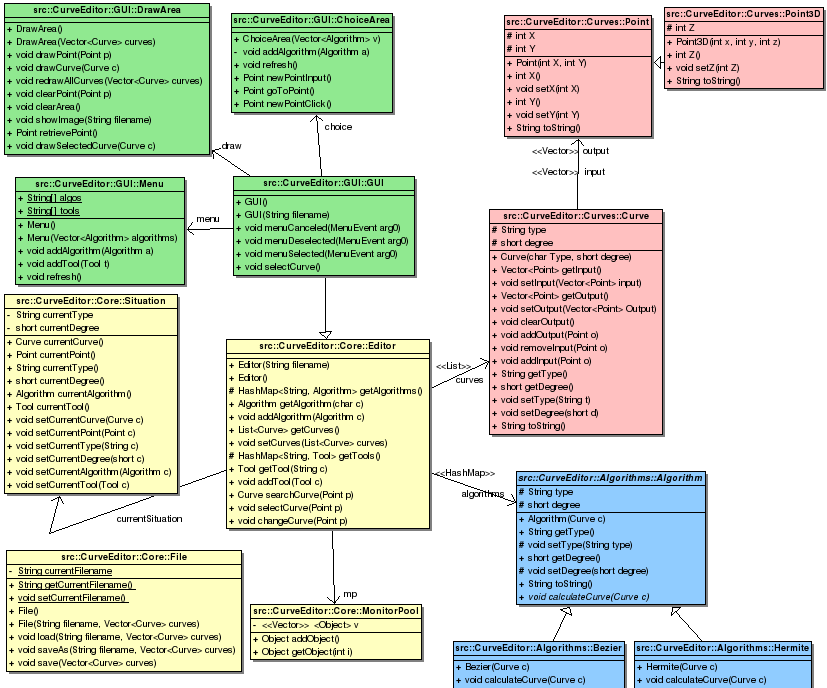
\includegraphics[scale=0.50]{uml.png}
\caption{Het voorlopig UML-diagram.}
\end{figure}
\clearpage

\subsection{ADT's}
Point en Point3D spreken voor zich: zij representeren punten in het vlak of in de ruimte voor door middel van de co\"ordinaten.

Curve bevat enerzijds een Vector van Points, die de verzameling van de initi\"ele controlepunten voorstelt. Wij hebben voor een Vector gekozen, omdat de volgorde van die punten heel belangrijk is. Anderzijds bevat Curve een tweede Vector van Points, die de verzameling van de ge\"interpoleerde punten voorstelt; deze Vector wordt gevuld met behulp een functie van een Algorithm-instantie die de input-vector als parameter meekrijgt.

Algorithm is een abstracte klasse, daar de methode \it{calculate} \rm{in} de subklassen dient ge\"implementeerd te worden. Algorithms kunnen beschouwd worden als ADT's die curves cre\"eren aan de hand van een verzameling meegegeven punten.

In de centrale klasse Editor maken we gebruik van HashMaps voor het bijhouden van alle algoritmen en tools. Op deze manier kunnen we makkelijk en effici\"ent het nodige object vinden aan de hand van een String die de naam van de tool/algoritme voorstelt. Ook kunnen we met behulp van deze HashMaps eenvoudig de menu's aanmaken: gewoon voor elke key een menu-item aanmaken en dat item aan de overeenkomstige value koppelen.

\subsection{Bestandstructuur}
Hier kunnen we kort over zijn. Meer dan de op het moment van opslaan weergegeven curves moet er eigenlijk niet opgeslaan worden, daar hieruit alles weer kan gereconstrueerd worden; deze curves kunnen we binair wegschrijven, of tekstueel om ze daarna terug te gaan parsen naar de juiste curve. Beide aanpakken vergen niet meer dan alle elementen van de Vector curves in de klasse Editor wegschrijven en terug inladen.

\section{Taakverdeling en planning}
Planning: 


\end{document} 